\section{Bornes de présentation Somfy}

\subsection{Somfy}

Somfy est un entreprise concevant des systèmes domotiques à l'attention du grand public.
Dans une démarche de communication, Somfy a contacté LTBL pour la creation de 11 bornes interactives qui seront mises en palce dans les magasins vendant les produits de la marque.

\subsection{Besoins}

L'objectif de ce projet est de concevoir et de produire 11 machines permettant d'afficher des informations sur l'entreprise et ses produits.
Ces informations peuvent être des vidéos, du texte ou des images.

Dans ce projet, je n'ai pas travaillé sur le développement de l'application de présentation mais sur la mise en place des 11 machines permettant son execution.
Ces 11 machines devaient presenter un système de visionnage pour réduire au maximum les possibilités de l'utilisateur.

\subsection{Recherches et choix du système}

Pour changer des habitudes et pour réduire les coups de license, nous avons choisis d'utiliser une distribution Linux gratuite pour l'execution des applications sur les bornes.
Nous avons fait ce choix d'une pars pour le faible coup du système mais aussi pour la grande flexibilité de celui-ci.
En effet, il est simple de mettre en place un système captif sur une machine linux car on contrôle chaque élément de l'OS .

Pour le système j'ai penché vers un membre de la famille Ubuntu pour sa stabilité et la grande communuté qui se forme autour.

J'ai alors découvert Ubuntu Core qui permet la creation de système embarqués et minimalistes.
Ubuntu Core est une varante de Ubuntu se basant sur des paquets unitaire séparés les uns des autres.
Cela permet de séparer chaque application et d'autoriser leur communication sur certains canaux particulier appelés interfaces.
Ce système rapelle beaucoup les systèmes mobiles comme Android ou IOS exigeant des permissions définies à l'avance pour que les applications aient acces à certaines fonctionnalités.
Ubuntu Core utilise Snapcraft, un gestionnaire de paquet permettant cette séparation des applications.
De pars sa complexitée et de l'abscense de serveur X sur snapcraft, je n'ai pas retenu cette solution et me suis penché sur Ubuntu Server.

Ubuntu Server est une version de Ubuntu sans les composants de bureau classique.
Il permet de composer son propre système sans la lourdeur des applications graphiques inutiles dans le contexte des bornes Somfy.
J'ai donc choisi cette distribution ayant pour objectif d'installer un environnement de bureau manuellement.

\subsection{Environnement de kiosk}

Pour mettre en place l'environnement d'affichage, j'ai commencé par installer le serveur X .
Le serveur X est le logiciel en charge d'afficher l'interface à l'utilisateur au travers d'un protocol spécifique.

Apres avoir installé ce logiciel, il faut installer un système de gestion de fenètres qui sera en charge d'afficher les différentes fenêtre à la bonne taille et dans le bon contexte.
Pour le gestionnaire de fenêtres, j'ai choisi xfce car il est légé et propose beaucoup de fonctionnalités.
Le gestionnaire de fenêtre est essentiel car il permet aux applications de correctement se dimentionner et de passer en plein ecran pour empècher l'utilisateur d'éfféctuer des actions non désirés.

Enfin, on peut installer notre application et la demarrer.

Il faut bien sur automatiser tout cela pour que l'ensemble puisse se démarrer automatiquement en même temps que la machine pour éviter tout action manuelle de l'installateur.
Pour ce faire j'ai été amené a modifier le pipeline de démarrage du système.
Tout d'abord il faut créer un nouvel utilisateur qui sera en charge d'executer l'application pour eviter qu'elle ne soit éxécuté en tant qu'administrateur.
Ensuite, il faut modifier le comportement de connexion sur la première console pour qu'elle se connecte automatiquement avec l'utilisateur en charge de l'execution du programme.
L'utilisateur connecté, on execute le script de démarrage qui se charge de démarrer le sreveur X, le gestionnaire de fenêtres et l'application.

Nous disposons alors d'un système de kiosk fonctionnel et sécurisé.

\subsection{Système de mise à jour}

Pour permettre un mise à jour de l'application simplifiée j'ai été amené a rélféchir sur un système de mise à jour.
Il n'est pas possible de connecter la borne a internet et cela implique que l'on ne peut pas mettre à jour a distance.
Il fallait donc trouver un solution permettant de changer les fichiers de l'application sans pour autant nécéssiter la rapatriement des bornes chez LTBL .

Pour ce système j'ai choisi d'utiliser un ensemble de scripts bash permettant d'avoir un grand contrôle sur le système avec un système de scripting simple et rapide.

Le système de mise à jour que j'ai mise en place se compose de 3 elements clés

\paragraph{Watching USB} Linux dispose d'un système de gestion des périphériques appelé \texttt{udev}.
Ce système permet de gerer le connexion, la déconnexion et le montage des elements amovibles du système.
En ajoutant des rêgles dans le fichier de configuration spécifique de udev, on peut executer une commande lors de la connexion ou la déconnexion d'un périphérique amovible.
J'ai utilisé cette fonctionnélité pour vérifier si le support contien une mise à jour et lancer l'installation de la mise à jour dans ce cas.

\paragraph{Fichier de verrouillage} Lors d'une mise à jour, le script installant cette mise àjour créer un fichier \texttt{update.lock} a la racine de l'application permettant d'indiquer que'une mise à jour est en cours.
Il arrete alors de force l'application en cours d'éxécution pour l'installation de la mise à jour.
On ajoutera alors au fichier \texttt{update.lock} les logs de toute la mise à jour pour suivre en temps reel sont déroulement.

\paragraph{Scripts de mise à jour} Pour éviter que l'on puisse executer du code arbitraire en tant qu'administrateur sur la machine, seul un nombre limité d'actions peuvent être éfféctués durant une mise à jour.
Chaque action représente un script dans le dossier \texttt{update} à la racine de l'application.
chaque action dispose de ses paramètres.

\medskip

Chque mise à jour de l'application passe donc par un support amovible ce qui permet à n'importe quel personne de l'effectuer.
Ce support amovible contien un fichier \texttt{update.conf}, un fichier texte décrivant pas à pas la procedure à adopter.
Seul les actions disponibles sur la machine peuvent être éxécutés, a procedure n'est donc pas composée de commandes bash mais de nims de scripts présents dans le fichier \texttt{update}.
Chaque mise à jour est aussi asosciée à un numéro de version présent dans le fichier \texttt{update.version}.
Ce fichier est vérifier et sera copié à la fin de la mise à jour a la racine de l'application pour ne pas faire deux fois les mêmes opérations.

%TODO donner un exemple de conf

\subsection{Materiel \& Installation}

Les machines en charge d'héberger l'appliction sont des NUC d'intel.
Les NUC sont des mini machines crées par Intel et disposant d'un processeur directement soudés sur la carte mêre.
Ces machines on l'avantage d'être trés compact.

\begin{figure}[h]
    \centering
    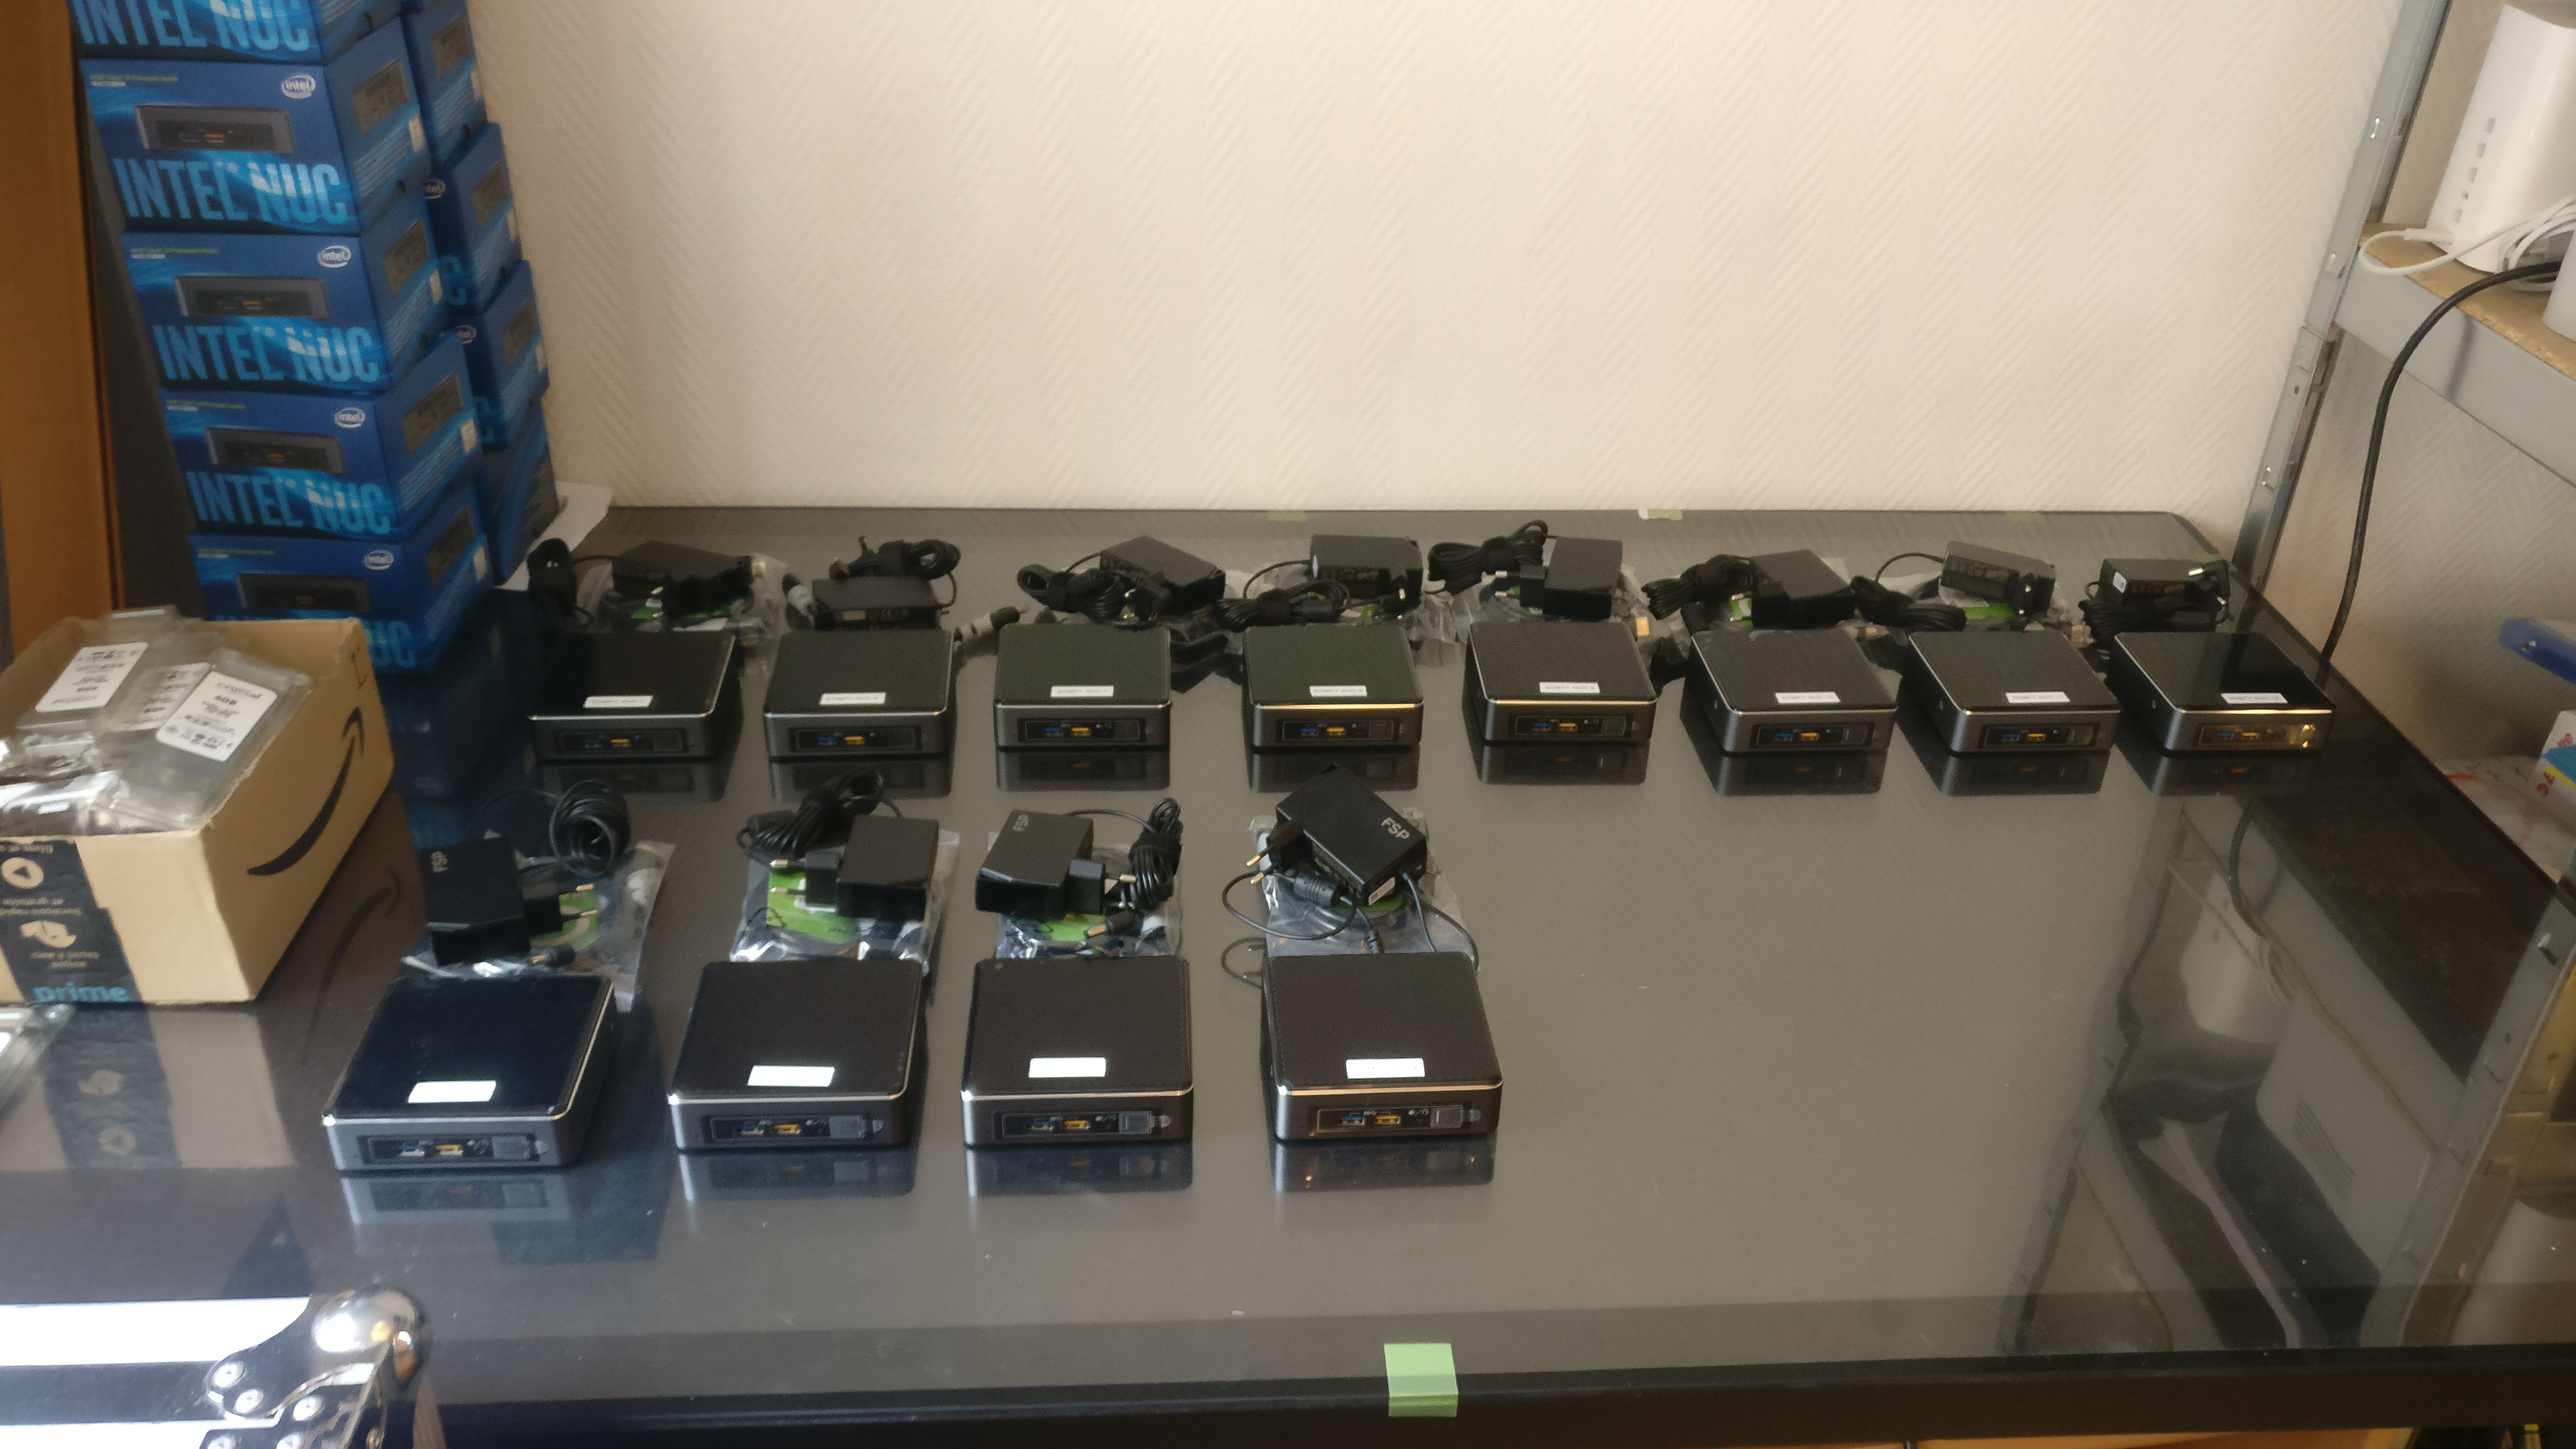
\includegraphics[scale=0.1]{img/somfy-nuc.jpg}
    \caption{Les 12 NUC hebergeant l'application de présentation}
\end{figure}

J'ai donc installé le système sur une machine que l'on apellera master.
J'ai ensuite utilisé CloneZilla pour faire une image du disque de cette machine et pouvoir la répliquer.

Apres l'installation, nous avons trouvé quelques problèmes qui devaient être corrigés.
N'ayant pas le temps de réinstaller un clone sur toutes les machines, nous avons mis en réseau toutes les machines.
En réseau, il suffit alors d'utiliser \texttt{cssh} pour éfféctuer les mêmes actions en sychronisé sur toutes les machines.
\texttt{cssh} est un utilitaire permettant de créer un certain nombre de terminaux ssh tous synchronisés;
Il est alors aisé d'administrer un ensemble de machines en même temps.

\begin{figure}[h]
    \centering
    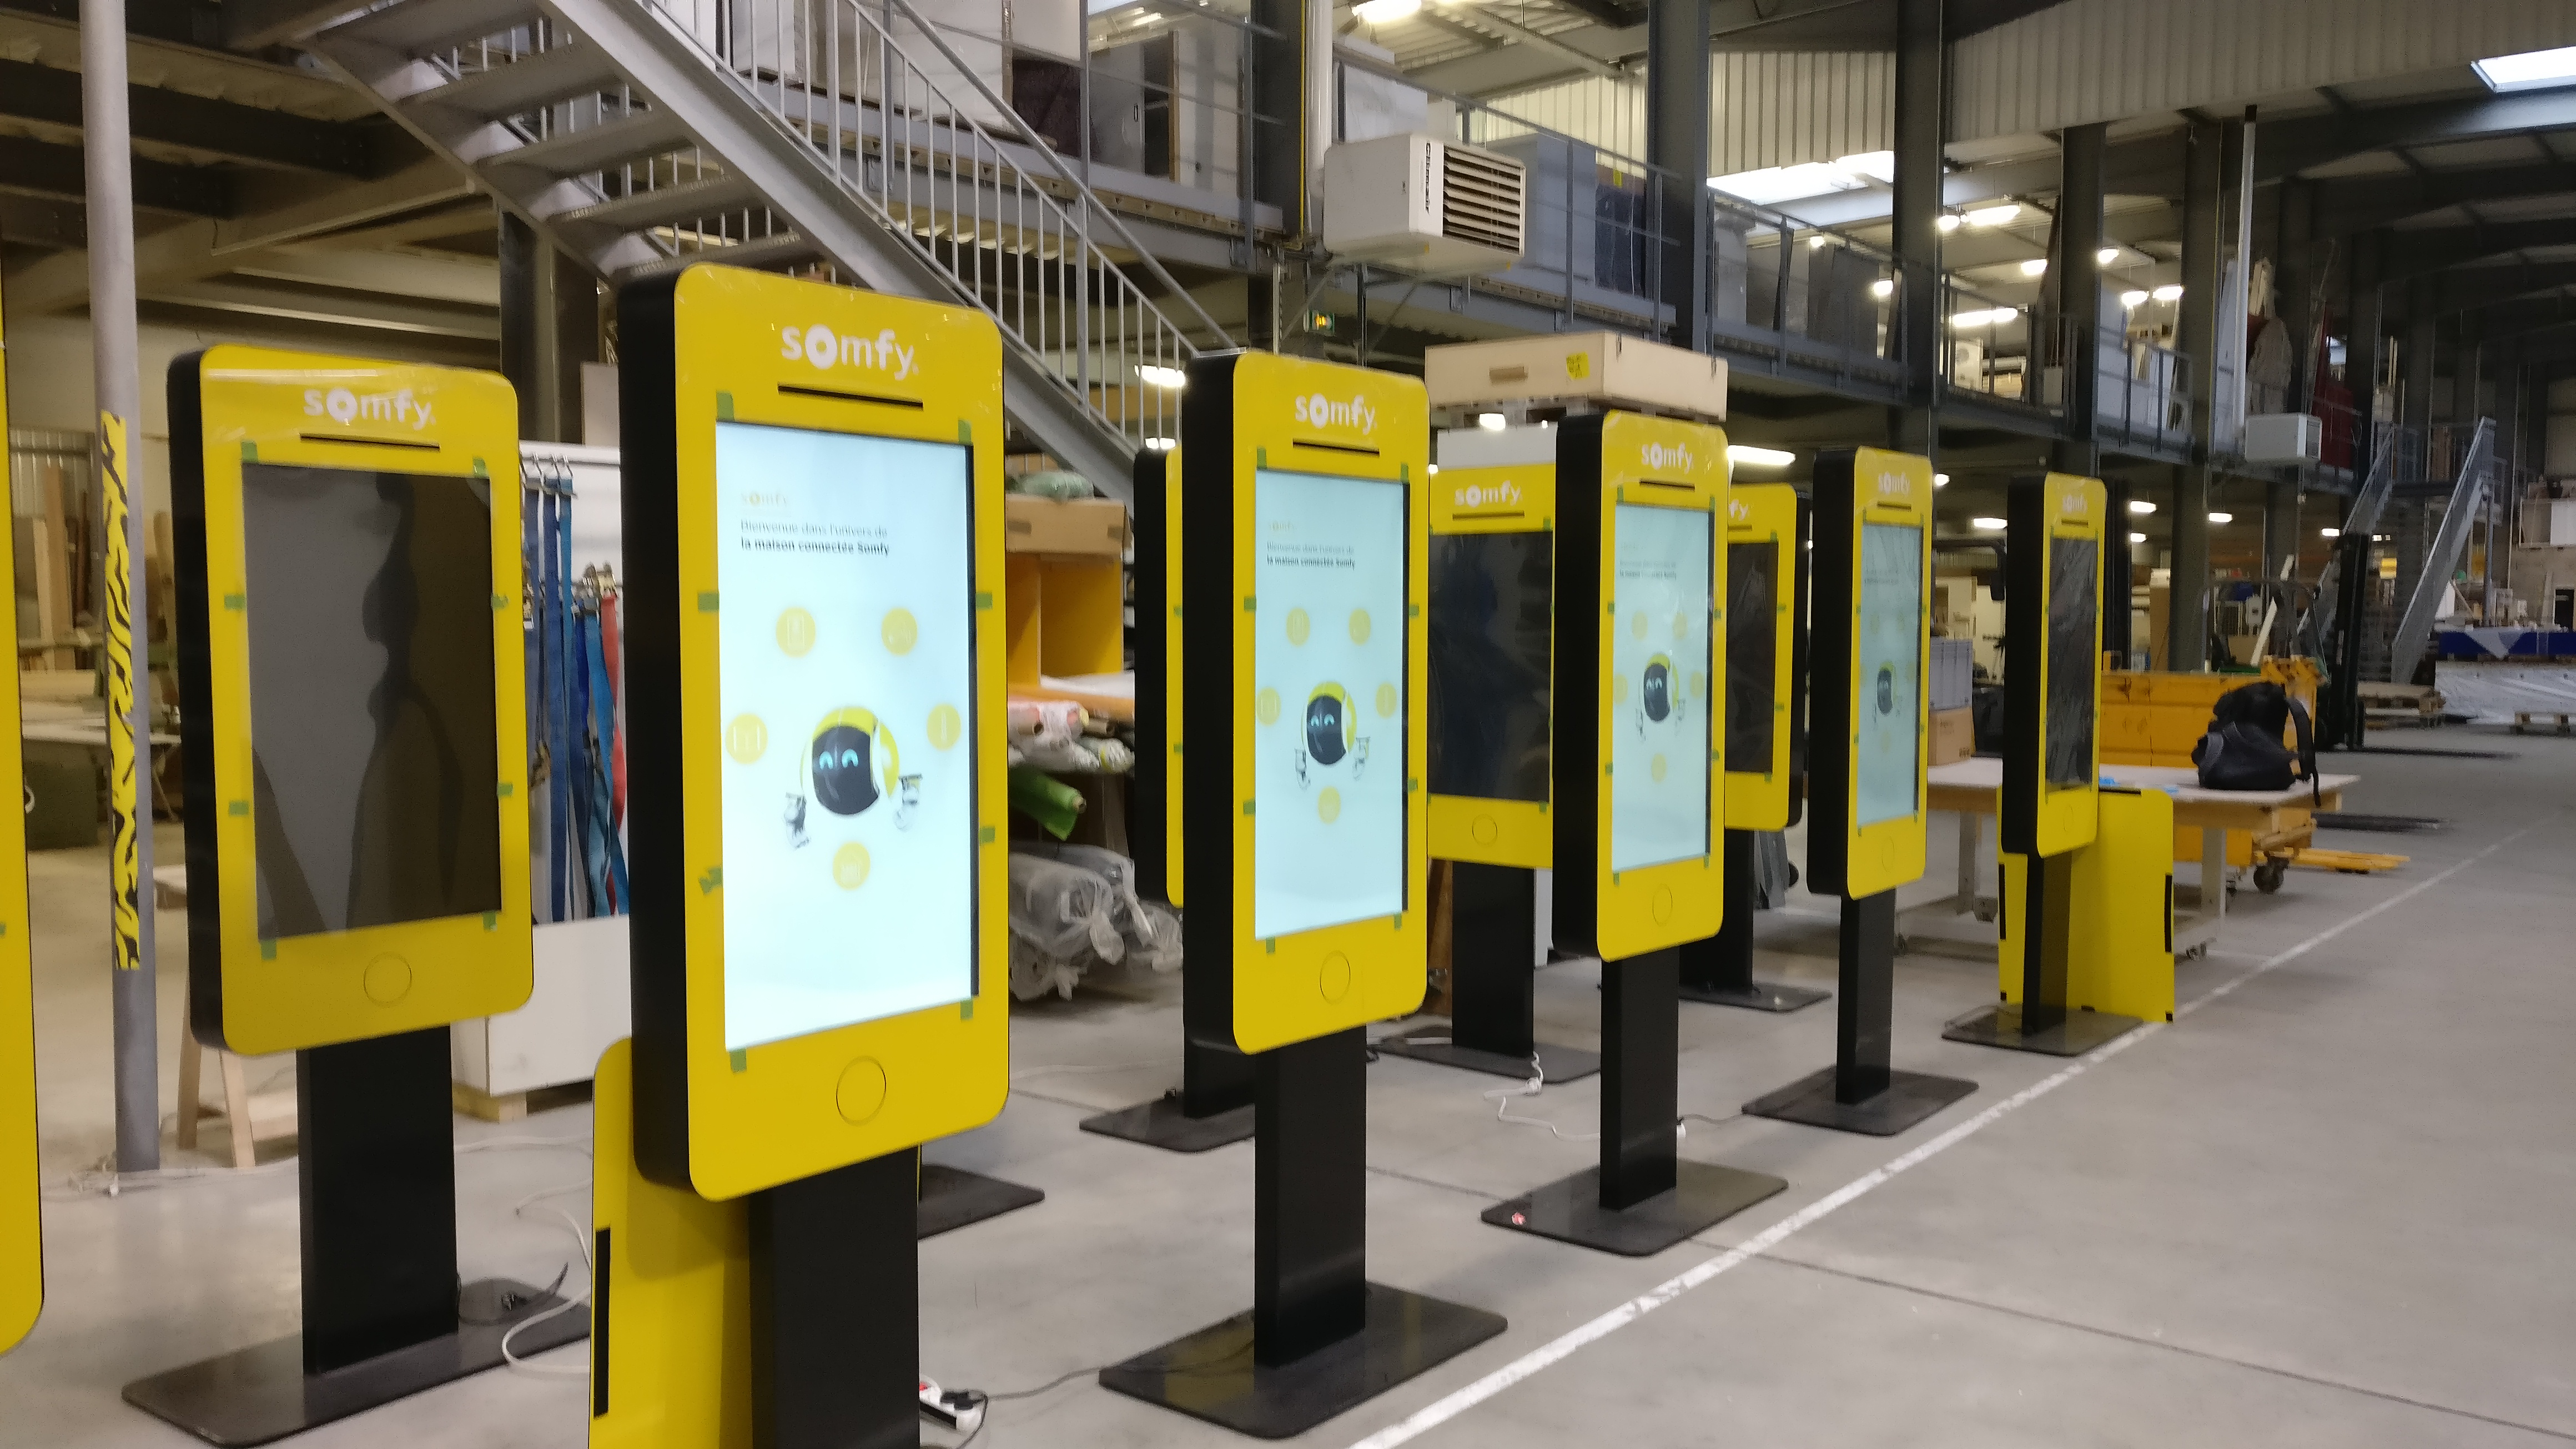
\includegraphics[scale=0.1]{img/somfy-install.jpg}
    \caption{Bornes Somfy lors de l'installation des machines dans leurs abitacles}
\end{figure}

\subsection{Conclusion}

Ce projet fut interessant car il m'a permis de me plonger plus en profondeur sur les composants d'un système linux pour controler son focntionnement.
Malgré la grande partie de recherche pour dégager la meilleur solution, j'ai quand mee eu l'occasion de travailler surn un système de mise à jour innovant.
Le projet est à présent terminé et les bornes ont été disposés dans les magasins vendant la technologie Somfy.